\documentclass{standalone}
\usepackage{tikz}
\usetikzlibrary{decorations.pathreplacing,decorations.pathmorphing}
\usetikzlibrary{fit,quotes}
\usepackage{yquant, braket}

\begin{document}

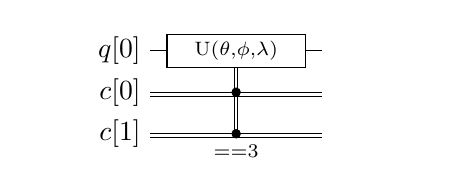
\begin{tikzpicture}[scale=1.000000,x=1pt,y=1pt]
\filldraw[color=white] (0.000000, -7.500000) rectangle (62.000000, 37.500000);
% Drawing wires
% Line 2: q0 W q[0]
\draw[color=black] (0.000000,30.000000) -- (62.000000,30.000000);
\draw[color=black] (0.000000,30.000000) node[left] {$q[0]$};
% Line 3: c0 W c[0]
\draw[color=black] (0.000000,15.000000) -- (62.000000,15.000000);
\draw[color=black] (0.000000,15.000000) node[left] {$c[0]$};
% Line 4: c1 W c[1]
\draw[color=black] (0.000000,0.000000) -- (62.000000,0.000000);
\draw[color=black] (0.000000,0.000000) node[left] {$c[1]$};
% Done with wires; drawing gates
% Line 5: q0 G {u($\theta$,$\phi$,$\lambda$)} c1  width=50 %% ==3
\draw (31.000000, -.500000) node[text width=144pt,below,text centered] {\scriptsize ==3};
\draw (30.5000000,30.000000) -- (30.5000000,0.000000);
\draw (31.5000000,30.000000) -- (31.5000000,0.000000);
\filldraw (31.000000, 15.000000) circle(1.500000pt); % extra dot
\begin{scope}
\draw[fill=white] (31.000000, 30.000000) +(-45.000000:35.355339pt and 8.485281pt) -- +(45.000000:35.355339pt and 8.485281pt) -- +(135.000000:35.355339pt and 8.485281pt) -- +(225.000000:35.355339pt and 8.485281pt) -- cycle;
\clip (31.000000, 30.000000) +(-45.000000:35.355339pt and 8.485281pt) -- +(45.000000:35.355339pt and 8.485281pt) -- +(135.000000:35.355339pt and 8.485281pt) -- +(225.000000:35.355339pt and 8.485281pt) -- cycle;
\draw (31.000000, 30.000000) node {\scriptsize{U($\theta$,$\phi$,$\lambda$)}};
\end{scope}
\filldraw (31.000000, 0.000000) circle(1.500000pt);
\draw[color=black] (0.000000,13.5000000) -- (62.000000,13.5000000);
\draw[color=black] (0.000000,-1.5000000) -- (62.000000,-1.5000000);
% Done with gates; drawing ending labels
% Done with ending labels; drawing cut lines and comments
% Done with comments
\end{tikzpicture}
\end{document}
